%%%%%%%%%%%%%%%%%%%%%%%%%%%%%%%%%%%%%%%%%
%
% Optics and Radar -based observations
% Assignment 2
% Final Version
%%%%%%%%%%%%%%%%%%%%%%%%%%%%%%%%%%%%%%%%%

%----------------------------------------------------------------------------------------
%	DOCUMENT CONFIGURATIONS
%----------------------------------------------------------------------------------------

\documentclass{article}

\title{\textbf {Optics and Radar Based Observations} \\ Assignment 2\\ Pulse Modulation Techniques} % Title
\def\authorivan{Ivan \v Sinkarenko}
\def\authoranu{Anuraj Rajendraprakash}
\author{\authorivan\\\authoranu}

\usepackage{graphicx}
\usepackage{fullpage}
\usepackage{url}

% load package with ``framed'' and ``numbered'' option.
\usepackage[framed,numbered,autolinebreaks,useliterate]{mcode}

\begin{document}

\maketitle % Insert the title, author and date

\centerline{Referee: Dr. Anita Enmark}

%\vspace{10mm}
%\begin{figure}[h!]
%\centering
%\centerline{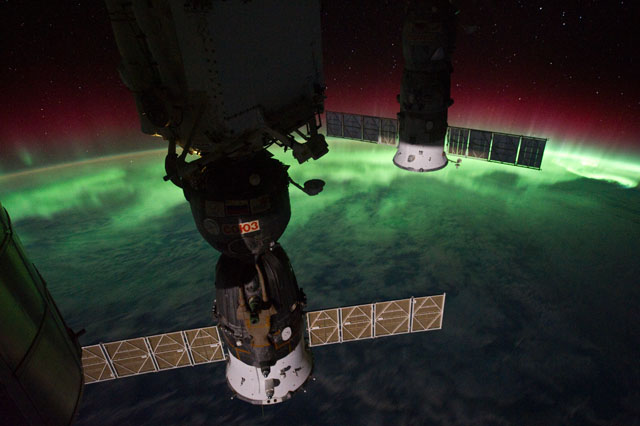
\includegraphics[width=\textwidth]{Figures/iss.jpg}}
%\label{fig:iss}
%\end{figure}

\setlength\parindent{0pt} % Removes all indentation from paragraphs

\renewcommand{\labelenumi}{\alph{enumi}.} % Make numbering in the enumerate environment by letter rather than number (e.g. section 6)
\clearpage

\tableofcontents

\listoffigures

\clearpage

%----------------------------------------------------------------------------------------
%	SECTION 1. Introduction
%----------------------------------------------------------------------------------------

\section{Introduction}
Mesosphere-Stratosphere-Troposphere (MST) radars are applied to study winds, waves, turbulence and in-stability in the atmosphere. They usually operate near 50 MHz and also called very high frequency (VHF) radars (with frequency band between 30 MHz and 300 MHz).\\
\\
ESRAD (ESrange RADar) is VHF MST radar located in northern Sweden (67$^{\circ}$56'N, 21$^{\circ}$04'E). The purpose of the radar is to provide information on the dynamic state of the atmosphere - winds, waves, turbulence and layering from the troposphere up to the lower thermosphere (1 km -100 km altitude). ESRAD operates at a frequency of 52 MHz corresponding to a wavelength of 5.77 m. The transmitter consists of 72 1-kW solid-state modules that are grouped into 12 6-kW power blocks. The resulting peak power output power is 72 kW and the maximum duty cycle is 5\%. Pulse repetition frequency rates from 100 Hz to 16 kHz are possible. Pulse lengths correspond to height resolutions between 150 m and 3 km. The radar is capable of pulse coding the transmitted signals using both Barker and complementary codes. The radar has 6 separate receivers for detection of backscattered signals from the atmosphere. \cite{Enmark:2012a2}.\\
\\
This assignment was carried out in order to analyze and understand the data from ESRAD MST Radar. Data from the ESRAD MST Radar was provided for the assignment. The central objective of the assignment was to observe the height resolution obtained from the given data. The height resolution obtainable with atmospheric radar is limited by the need to transmit a pulse of finite length. Since atmospheric properties change significantly within a few 10s a pulse should be as short as possible. However, the strength of the signal obtained from the atmosphere is proportional to the pulse length. Since the signal should be as strong as possible to be easily detectable above the natural noise, the radar pulse should be as long as possible. In practice we must always choose some compromise between these two conflicting demands.\\
\\
In order to the height resolution analysis it is important to understand the autocorrelation and ambiguity functions and use it to study and compare the properties of different types of signals like long pulses, short pulses, phase coding with Barker codes and complementary codes, and frequency coding with Linear Frequency Modulation (LFM). This is carried out in the first part of the assignment.\\
\\
The second part of the assignment has two subparts. The first part involves the analysis of the height resolution from the given data without any pulse coding techniques. In the second subpart the analysis of Barker and complementary coding techniques, based on given data for Signal-to-Noise ratio (SNR) and horizontal wind velocity and direction, is carried out. 
 
%----------------------------------------------------------------------------------------
%	SECTION 2. Part 1
%----------------------------------------------------------------------------------------

\section{Part 1}
\label{sec:part1}
\subsection{Ambiguity Functions}

In pulsed radar and sonar signal processing, an ambiguity function is a two-dimensional function of time delay and Doppler frequency $\chi(\tau,f)$ showing the distortion of a returned pulse due to the receiver matched filter (commonly, but not exclusively, used in pulse compression radar) due to the Doppler shift of the return from a moving target. The ambiguity function is determined by the properties of the pulse and the matched filter, and not any particular target scenario. For a given complex baseband pulse $s(t)$ the narrow ambiguity function is given by \cite{Wiki:2012ambi} $$\chi(\tau,f)= \int_{-\infty}^{+\infty} s(t) s^{*}(t-\tau) e^{-i2 \pi ft} dt$$

\subsection{Autocorrelation Functions}
Autocorrelation is the cross-correlation of a signal with itself. Informally, it is the similarity between observations as a function of the time separation between them. It is a mathematical tool for finding repeating patterns, such as the presence of a periodic signal which has been buried under noise, or identifying the missing fundamental frequency in a signal implied by its harmonic frequencies. It is often used in signal processing for analysing functions or series of values, such as time domain signals. \cite{Wiki:2012auto}
\\
\\
In order to have high range resolutions, the use of short pulses is important in radar applications. However there are several limitations to the use of short pulses. The bandwidth of a short pulse is large because the bandwidth is inversely proportional to the pulse width. A large bandwidth of the signal makes the radar system complex, places greater demand on the signal processing and increases the chances of interference with other electromagnetic signals. A large bandwidth also reduces the dynamic range of the receiver because the noise power is proportional to the bandwidth. Also the short pulses don't have high resolution in the doppler frequency measurement. Short pulses also places more demands on transmitter peak power. \cite{Skolnik:2001irs}\\
\\
Pulse compression is a technique which allows the radar to simultaneously achieve the energy of a long pulse and the resolution of a short pulse by avoiding the use of high peak power which is needed in high energy short duration pulse. In this method a long pulse is made to have the same bandwidth as a short pulse by modulation it in frequency or phase. \cite{Skolnik:2001irs}\\
\\

\subsection{Analysis of the properties of different signals}

Figure \ref{fig:long_pulse_data} and Figure \ref{fig:long_pulse_3d} show the autocorrelation and ambiguity function of a long pulse. For a square pulse response is centered around origin. There is no response outside the the width $\tau$, which is observed both in the autocorrelation and ambiguity function plots. The time delay measurement error is proportinal to the pulse width and the frequency measurement error is proportional to the inverse of the pulse width. Thus the frequency measurement accuracy for a long pulse would be good while the time delay measurement accuracy would be worse. Hence the doppler tolerance for a long pulse is better at the cost of range resolution which is poor. \cite{Skolnik:2001irs}\\
\\
\begin{figure}[h]
\begin{minipage}[t]{0.5\linewidth}
\centering
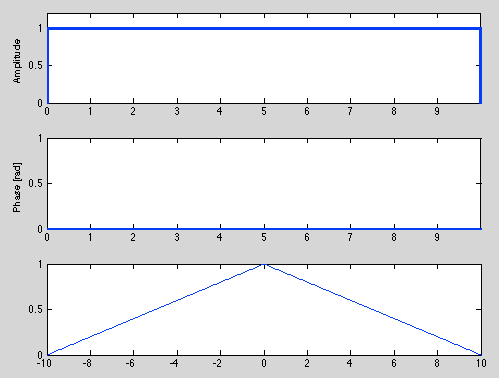
\includegraphics[width=8cm]{Figures/long_pulse_data.png}
\caption{Autocorrelation function of a long pulse.}
\label{fig:long_pulse_data}
\end{minipage}
\begin{minipage}[t]{0.5\linewidth}
\centering
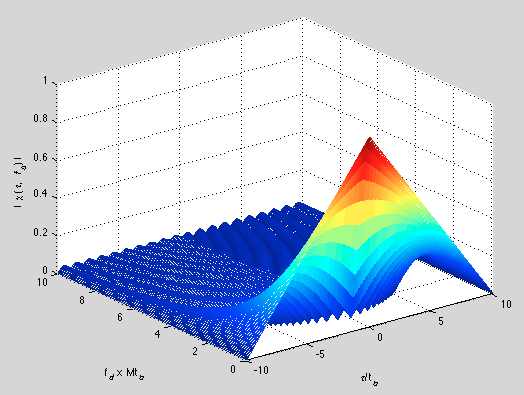
\includegraphics[width=8cm]{Figures/long_pulse_3d.png}
\caption{Ambiguity function of a long pulse.}
\label{fig:long_pulse_3d}
\end{minipage}
\end{figure}

\begin{figure}[tbh]
\begin{minipage}[t]{0.5\linewidth}
\centering
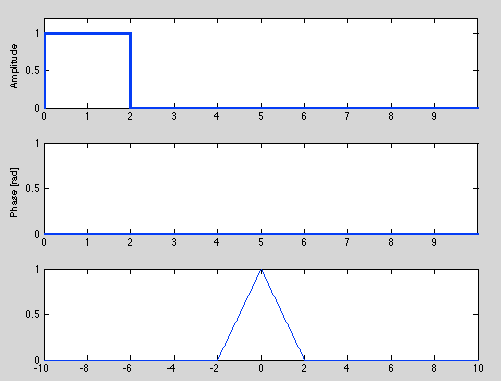
\includegraphics[width=8cm]{Figures/short_pulse_data.png}
\caption{Autocorrelation function of a short pulse.}
\label{fig:short_pulse_data}
\end{minipage}
\begin{minipage}[t]{0.5\linewidth}
\centering
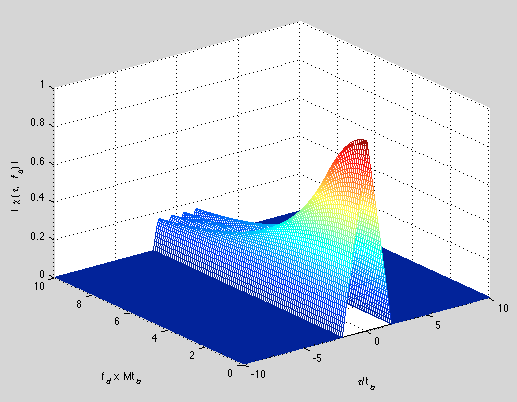
\includegraphics[width=8cm]{Figures/short_pulse_3d.png}
\caption{Ambiguity function of a short pulse.}
\label{fig:short_pulse_3d}
\end{minipage}
\end{figure}

\begin{figure}[tbh]
\begin{minipage}[t]{0.5\linewidth}
\centering
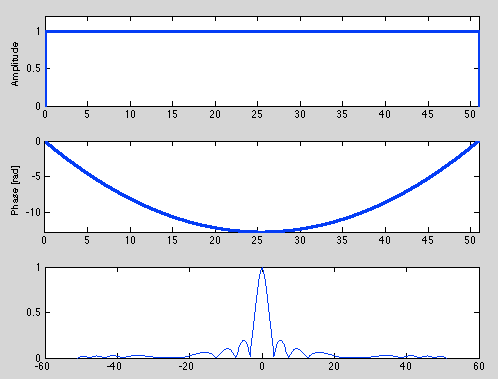
\includegraphics[width=8cm]{Figures/lfm_data.png}
\caption{Autocorrelation function of frequency coding with LFM.}
\label{fig:lfm_data}
\end{minipage}
\begin{minipage}[t]{0.5\linewidth}
\centering
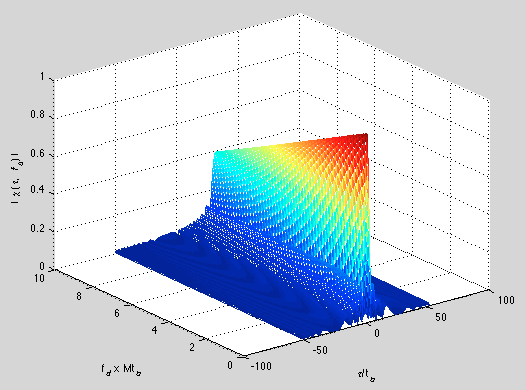
\includegraphics[width=8cm]{Figures/lfm_3d.png}
\caption{Ambiguity function of frequency coding with LFM.}
\label{fig:lfm_3d}
\end{minipage}
\end{figure}

\begin{figure}[t!]
\begin{minipage}[t]{0.5\linewidth}
\centering
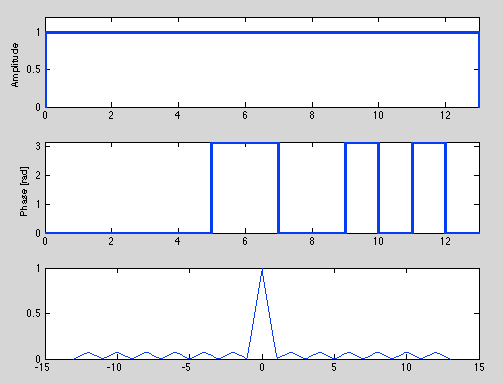
\includegraphics[width=8cm]{Figures/barker_data.png}
\caption{Autocorrelation function of Barker coding}
\label{fig:barker_data}
\end{minipage}
\begin{minipage}[t]{0.5\linewidth}
\centering
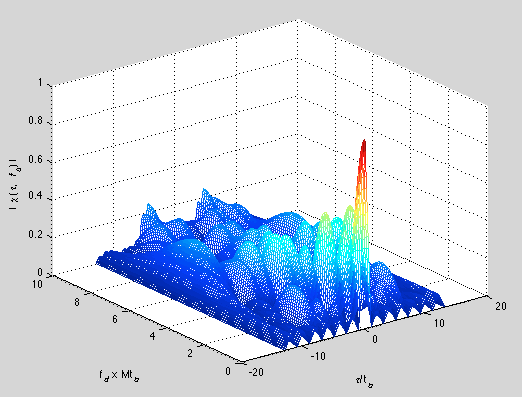
\includegraphics[width=8cm]{Figures/barker_3d.png}
\caption{Ambiguity function of Barker coding}
\label{fig:barker_3d}
\end{minipage}
\end{figure}

\begin{figure}[t!]
\begin{minipage}[t]{0.5\linewidth}
\centering
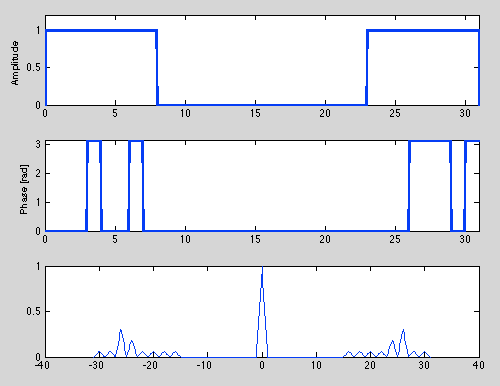
\includegraphics[width=8cm]{Figures/complementary_data.png}
\caption{Autocorrelation function of complementary coding}
\label{fig:complementary_data}
\end{minipage}
\begin{minipage}[t]{0.5\linewidth}
\centering
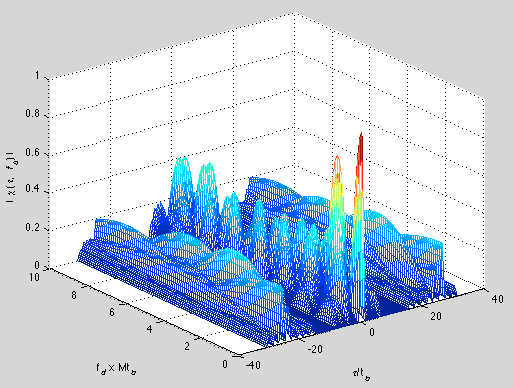
\includegraphics[width=8cm]{Figures/complementary_3d.png}
\caption{Ambiguity function of complementary coding}
\label{fig:complementary_3d}
\end{minipage}
\end{figure}
Figure \ref{fig:short_pulse_data} and Figure \ref{fig:short_pulse_3d} show the autocorrelation and ambiguity function of a short pulse. As it can be seen in Figure \ref{fig:short_pulse_data} and Figure \ref{fig:short_pulse_3d}, the response is centered around origin. There is no response outside the the pulse width $\tau$. Thus the doppler frequency measurement accuracy for a long pulse would be worse while the time delay measurement accuracy would be good. This implies a bad doppler tolerance and a good range resolution.\cite{Skolnik:2001irs}\\
\\
Thus it can be said if a good range resolution is required then a short pulse should be used and if a good doppler frequency resolution is required a long pulse should be used as it is more doppler tolerant.\\

Figure \ref{fig:lfm_data} and Figure \ref{fig:lfm_3d} show the autocorrelation and ambiguity function of the LFM signal. In such a signal the time delay measurement accuracy is proportional to the inverse of the bandwidth and the frequency measurement accuracy is proportional to inverse of the pulse width.  The pulse width and the bandwidth are independant of each other and hence the time delay and frequency measurement accuracy are also independent of each other. Thus a good range resolution can be obtained with a LFM pulse without a loss in the doppler tolerance as both can be independantly choses as required.\\
\\
One of the ways of increasing the bandwidth of a long pulse for the purpose of pulse compression, is by changing the phase. A long pulse of duration T is divided in to N subpulses of width $\tau$. The bandwidth is increased by changing the phase of each subpulse. A common form of phase change is \textit{binary phase coding}, in which the phases are made either 0 or $\pi$ according to a specified criterion. If the 0 and $\pi$ phase selection are made at random then the time side lobes have higher magnitude. But some sequences of phases change make the magnitude of side lobes smaller. Two good sequences of side lobe suppression are 
\begin{itemize}
\item Barker Coding
\item Complementary Coding
\end{itemize} 

Barker codes are a set sequences of 0 and $\pi$ phases for the subpulses so that the side lobes have lower peak values. If the barker codes are used for the phases of the subpulses then all the time side lobes have equal magnitude.\cite{Skolnik:2001irs}. The Figure \ref{fig:barker_data} and Figure \ref{fig:barker_3d} show the autocorrelation and the ambiguity function plots of a long pulse compressed by barker coding. It can be inferred that the doppler frequency tolerance would be good because of lower side lobes in the ambiguity diagram. Also the main lobe is centered around the origin because the long pulse has been compressed by Barker Coding and hence a good range resolution would also be obtained.\\

The autocorrelation and the ambiguity function plot of a long pulse compressed with complementary coding is shown in Figure \ref{fig:complementary_data} and Figure \ref{fig:complementary_3d} respectively. Using the complementary codes for the phase selections is another method of achieving pulse compression. In this coding method, pairs of equal length phase-coded pulses are chosen so that the side lobes of the autocorrelation function of one are the negative of the other. In complemenatary coding  the autocorrelation function from the outputs of the two matched filters are added. This results in the algebraic sum of the side lobes being zero and the main response being 2N where N is the number of subpulses. Thus because of side lobe being null in this type of pulse compression the doppler tolerance is good and also as the main lobe being centered around origin it yields good range resolution.

%----------------------------------------------------------------------------------------
%	SECTION 3. Part 2
%----------------------------------------------------------------------------------------

\section{Part 2}

%----------------------------------------------------------------------------------------
%	SUBSECTION 3.1. Part 2A
%----------------------------------------------------------------------------------------

\subsection{Part 2A}

\begin{figure}[b!ht]
\centering
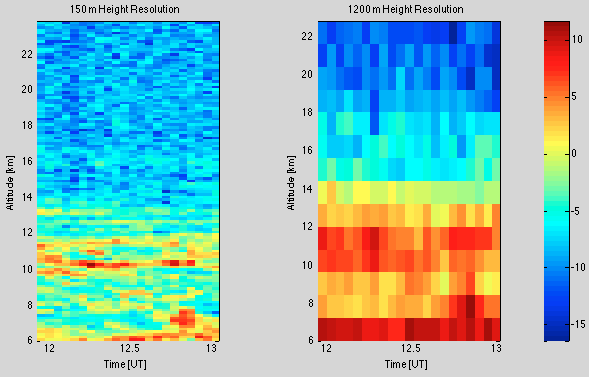
\includegraphics[width=0.7\textwidth]{Figures/height_res.png}
\caption{SNR data for 150 m and 1200 m height resolutions.}
\label{fig:height_res}
\end{figure}


When a weather radar is scanning in only one direction vertically, it obtains height resolution data along a vertical cut of the atmosphere. \cite{Wiki:2012wr} The height resolution obtainable with atmospheric radar is limited by the need to transmit a pulse of finite length. Since atmospheric properties change significantly within a few 10s a pulse should be as short as possible. However, the strength of the signal obtained from the atmosphere is proportional to the pulse length. Since the signal should be as strong as possible to be easily detectable above the natural noise, the radar pulse should be as long as possible. In practice we must always choose some compromise between these two conflicting demands. \cite{Enmark:2012a2}\\
\\
In this report, all the data plotted with Matlab was taken from the latest date available, that is 2008-10-15. Figure \ref{fig:height_res} shows the SNR from two different data files. On the left side there is a 150 m height resolution and on the right it is 1200 m height resolution. It is clearly seen that at a lower height the SNR is higher. Radar pulses spread out as they move away from the radar station. This means that the region of air any given pulse is moving through is larger for areas farther away from the station, and smaller for nearby areas, decreasing resolution at far distances. Naturally, resolution can be improved by newer equipment. \cite{Wiki:2012wr} However, the average SNR for the 150 m height is lower than for the 1200 m because deep blue color dominates on the left, whereas blue, cyan and orange amount is approximately equal on the right side.\\
\\
The gain in power is affected by the loss in resolution for the different altitudes. Therefore, it is more difficult to learn the environmental conditions on higher distances, because everything is smoothed out. Not only the coarser resolution of the radar blur the image but the sounding incorporate area that are echo free, thus adding some inaccuracy to the signature of the atmosphere. \cite{Wiki:2012wr}


%----------------------------------------------------------------------------------------
%	SUBSECTION 3.2. Part 2B
%----------------------------------------------------------------------------------------

\subsection{Part 2B}

\begin{figure}[t!]
\centering
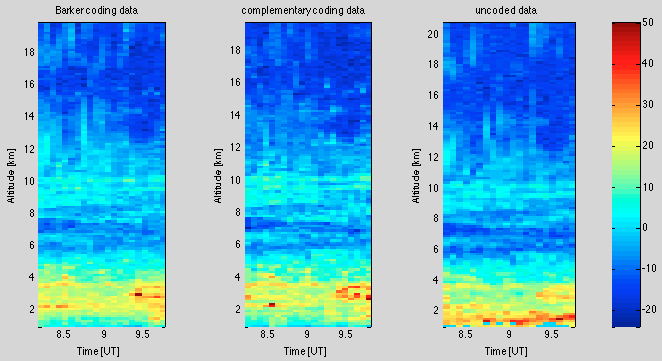
\includegraphics[width=0.9\textwidth]{Figures/SNR_coding.png}
\caption{SNR for Barker coded, complementary coded and uncoded data.}
\label{fig:SNR_coding}
\end{figure}

\begin{figure}[t!]
\centering
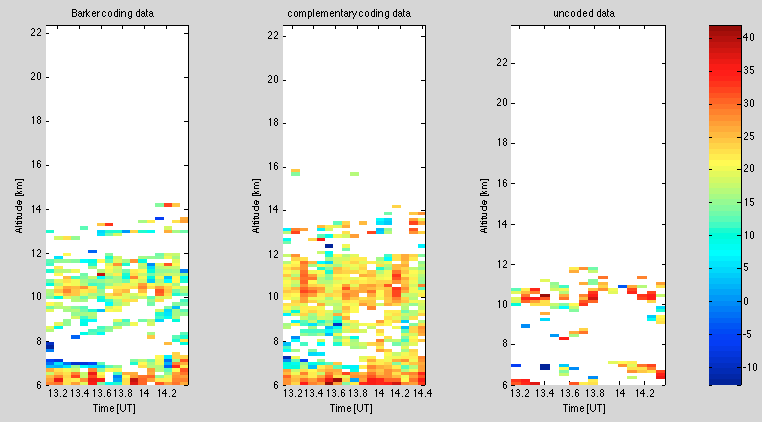
\includegraphics[width=0.9\textwidth]{Figures/direction.png}
\caption{Horizontal wind direction [deg] for Barker coded, complementary coded and uncoded data.}
\label{fig:direction}
\end{figure}



After selecting height resolution the pulse coding technique should be chosen to allow the effective height resolution to be reduced while retaining the echo-strength of a longer pulse. Figure \ref{fig:SNR_coding} has 3 color maps showing SNR for the Barker coding, complementary coding and uncoded data respectively. These techniques were already discussed in Section \ref{sec:part1}. The uncoded data on the right plot can be used as a reference. This plot has smallest variations among all three plots. The average SNR value on this plot floats at few dB with higher values in the bottom part and lower values in the upper right corner.\\


\begin{figure}[t!]
\centering
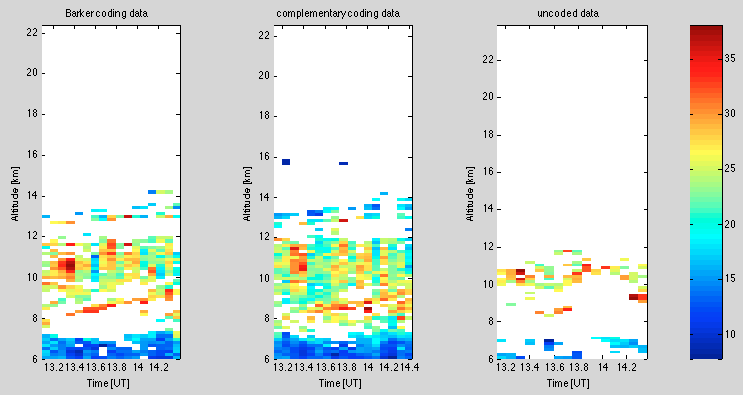
\includegraphics[width=0.9\textwidth]{Figures/velocity.png}
\caption{Horizontal wind velocity [m/s] for Barker coded, complementary coded and uncoded data.}
\label{fig:velocity}
\end{figure}


The complementary coding plot has greater SNR magnitude variations, whereas Barker coding tries to flatten this variations (blue part is lighter, bottom part contains less orange and red colors). As explained in Section \ref{sec:part1}, Barker coding removes side lobe peaks by introducing small variations along the entire width apart from the origin. That is exactly what is seen on the figure.\\
\\
The height resolution in all three plots remains the same. Thus, the pulse compression technique affects mainly the SNR magnitude. The selection of the particular technique usually depends on the needs of the application. In our case, Barker code is preferred because it seems to have smoother changes throughout the plot.\\
\\
In the next step, it is necessary to analyze horizontal wind direction and velocity from given data files. In atmospheric and Earth sciences wind is specified by terms zonal and meridional, which are describe directions on a globe. Zonal means "along a latitude circle" or "in the west–east direction", while meridional means "along a meridian" or "in the north–south direction". The horizontal wind is the resultant of these two components. \cite{Wiki:2012zm}\\ The 0$^{\circ}$ angle of the wind corresponds to the Eastward direction. A positive angle value directs the wind northern-wards and a negative value corresponds to southern direction accordingly.\\
\\
Unfortunately, data for the zonal and meridional wind components is not complete. It is not expected for Figure \ref{fig:direction} to have any specific pattern, because the wind currents change very fast and are considered random in this assignment. From the figure it is seen that in the lower altitudes wind blows more in the south-east direction, at the altitude of 5 km it is more to the east, while in varies between south-east and east and sometimes changes to north direction.\\
\\
From Figure \ref{fig:velocity} one can understand that in the lower altitudes, up to 8 km, the wind is much weaker than at 10-12 km. Also in the higher altitudes wind velocity variations are more significant, whereas lower altitudes have almost uniform pattern. Barker coding plot has smoother velocity variations than other plots.\\
\\
From both direction and velocity figures it is seen that complementary coding and Barker coding data files have the highest number of records. Uncoded data seems to be slightly poorer.

%----------------------------------------------------------------------------------------
%	SECTION 4. CONCLUSION
%----------------------------------------------------------------------------------------
\newpage
\section{Conclusion}

This assignment helped us gain a clear understanding of the autocorrelation function and the ambiguity function. We also analyzed the autocorrelation and ambiguity functions of various types of radar signals. This helped in getting a thorough idea of why certain types of signals are used in radar applications. The second part of the assignment helped us understand how radar is used for the weather analysis and how the data depends on different altitudes as well as the pulse compression techniques used.

%----------------------------------------------------------------------------------------
%	SECTION 5. REFERENCES
%----------------------------------------------------------------------------------------

\begin{thebibliography}{9}

\bibitem{Enmark:2012a2}
Enmark A.  (2012).
\newblock {\em Assignment 2. Pulse Modulation Techniques}.
\newblock Lule\aa \ University of Technology, Kiruna, Sweden.

\bibitem{Skolnik:2001irs}
Skolnik M. ~I.  (2001).
\newblock {\em Introduction to Radar Systems}.
\newblock The McGraw-Hill Companies, Inc., New York, United States.

\bibitem{Wiki:2012ambi}
Wikipedia.org. (2012).
\newblock {\em Ambiguity Function}.
\newblock {\url{http://en.wikipedia.org/wiki/Ambiguity_function}}.

\bibitem{Wiki:2012auto}
Wikipedia.org. (2012).
\newblock {\em Autocorrelation Function}.
\newblock {\url{http://en.wikipedia.org/wiki/Autocorrelation_function}}.

\bibitem{Wiki:2012wr}
Wikipedia.org. (2012).
\newblock {\em Weather Radar}.
\newblock {\url{http://en.wikipedia.org/wiki/Weather_radar}}.

\bibitem{Wiki:2012zm}
Wikipedia.org. (2012).
\newblock {\em Zonal and meridional}.
\newline
\newblock {\url{http://en.wikipedia.org/wiki/Zonal_and_meridional}}.



\end{thebibliography}


%----------------------------------------------------------------------------------------
%	SECTION 5. Appendix 2A
%----------------------------------------------------------------------------------------
\newpage
\section*{Appendix 1. Matlab code of Part 2A}

\subsection*{Part2A.m}
\lstinputlisting{Part2A.m}

\subsection*{plotSNR.m}
\lstinputlisting{plotSNR.m}

%----------------------------------------------------------------------------------------
%	SECTION 6. Appendix 2B
%----------------------------------------------------------------------------------------
\newpage
\section*{Appendix 2. Matlab code of Part 2B}

\subsection*{Part2B.m}
\lstinputlisting{Part2B.m}

\subsection*{plotWind.m}
\lstinputlisting{plotWind.m}

\subsection*{hypotenuse.m}
\lstinputlisting{hypotenuse.m}

\subsection*{radToDeg.m}
\lstinputlisting{radToDeg.m}

%----------------------------------------------------------------------------------------
%	SECTION 7. Confirmation
%----------------------------------------------------------------------------------------
\newpage
\section*{Confirmation of Participation}

This is to confirm that the members of this team participated on the investigation of the required information to solve the assignment, generated their code to perform the calculation and discussed the results.\\
\vspace{2cm}
\newline
\line(1,0){200}\\
\authorivan\\
\vspace{2cm}
\newline
\line(1,0){200}\\
\authoranu\\


\end{document}